\documentclass{standalone}
\usepackage{tikz}
\usepackage{ctex,siunitx}
\setCJKmainfont{Noto Serif CJK SC}
\usepackage{tkz-euclide}
\usepackage{amsmath}
\usetikzlibrary{patterns, calc}
\usetikzlibrary {decorations.pathmorphing, decorations.pathreplacing, decorations.shapes,}

\begin{document}
\small
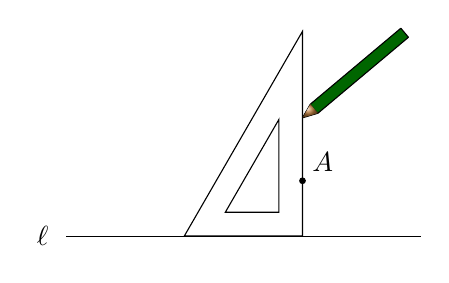
\begin{tikzpicture}[>=stealth,scale=1]
  \tkzSetUpPoint[fill=black]
  % \useasboundingbox(-1,-0.75)rectangle(3.7,1.4);
  \tkzDefPoints{1.5/0/A,0/0/C,1.2/0.3/A',1.2/0/Y,0/0.3/X,1.5/0.7/A''}
  \tkzDefPoint(60:3){B}
  \tkzDefPoint(-30:0.3){C''}
  \tkzDefPointBy[translation = from C to B](C'')\tkzGetPoint{B''}
  \tkzInterLL(A',X)(B'',C'')\tkzGetPoint{C'}
  \tkzInterLL(A',Y)(B'',C'')\tkzGetPoint{B'}
  \draw(A)--(B)--(C)--cycle;
  \draw(A')--(B')--(C')--cycle;
  \tkzDrawLines[add = 1.0 and 1.0](A,C)
  \tkzDrawPoints(A'')
  \tkzLabelPoint[above right](A''){$A$}
  \tkzLabelLine[pos=-1.2](C,A){$\ell$}
  \draw[fill=green!40!black,line join=round](1.5,1.5)--++(60:0.2)--++(40:1.5)--++(-50:0.15)--++(-140:1.5)--cycle;
  \fill[ball color=brown](1.5,1.5)--++(60:0.2)--++(-50:0.15)--cycle;
\end{tikzpicture}
\end{document}